\section{NHÀ TỐT (CHỢ TỐT)}
\subsection{Giới thiệu}
\hspace*{1cm} Nhà Tốt là một nền tảng được ra mắt bởi Chợ Tốt, là nền tảng mua bán sản phẩm và kết nối dịch vụ trực tuyến với 12 triệu người dùng cũng như 55 triệu lượt truy cập hàng tháng, cung cấp những dịch vụ liên quan đến bất động sản. Trang web được ra mắt với định hướng giúp tạo ra một giải pháp thuận tiện và nhanh chóng nhất để người mua và người thuê có thể tìm kiếm được bất động sản phù hợp nhất với nhu cầu của mình. Nơi đây, người sử dụng có thể tìm kiếm và có được những thông tin trực quan, đầy đủ về những loại hình bất động sản đa dạng, phổ biến. Vào tháng 3 năm 2023, đã có 500.000 bất động sản ở khắp các tỉnh thành được đăng tải trên nền tảng Nhà Tốt. \cite{nhatot}\\
\hspace*{1cm} Với giao diện sử dụng thân thiện và tính năng tìm kiếm linh hoạt, Nhà Tốt giúp người dùng dễ dàng tìm kiếm và đăng tin mua bán. Đặc biệt, trang web này tập trung vào việc tạo ra một thị trường trực tuyến đáng tin cậy, nơi mà người dùng có thể gặp gỡ và thực hiện giao dịch an toàn. Từ nhà ở, đất đai đến các sản phẩm và dịch vụ khác, Nhà Tốt mang lại trải nghiệm mua sắm đa dạng. Người dùng có thể dễ dàng tìm thấy những thông tin rao bán hoặc cho thuê một cách nhanh chóng và tiện lợi nhất.\\
\begin{figure}[H]
    \centering
    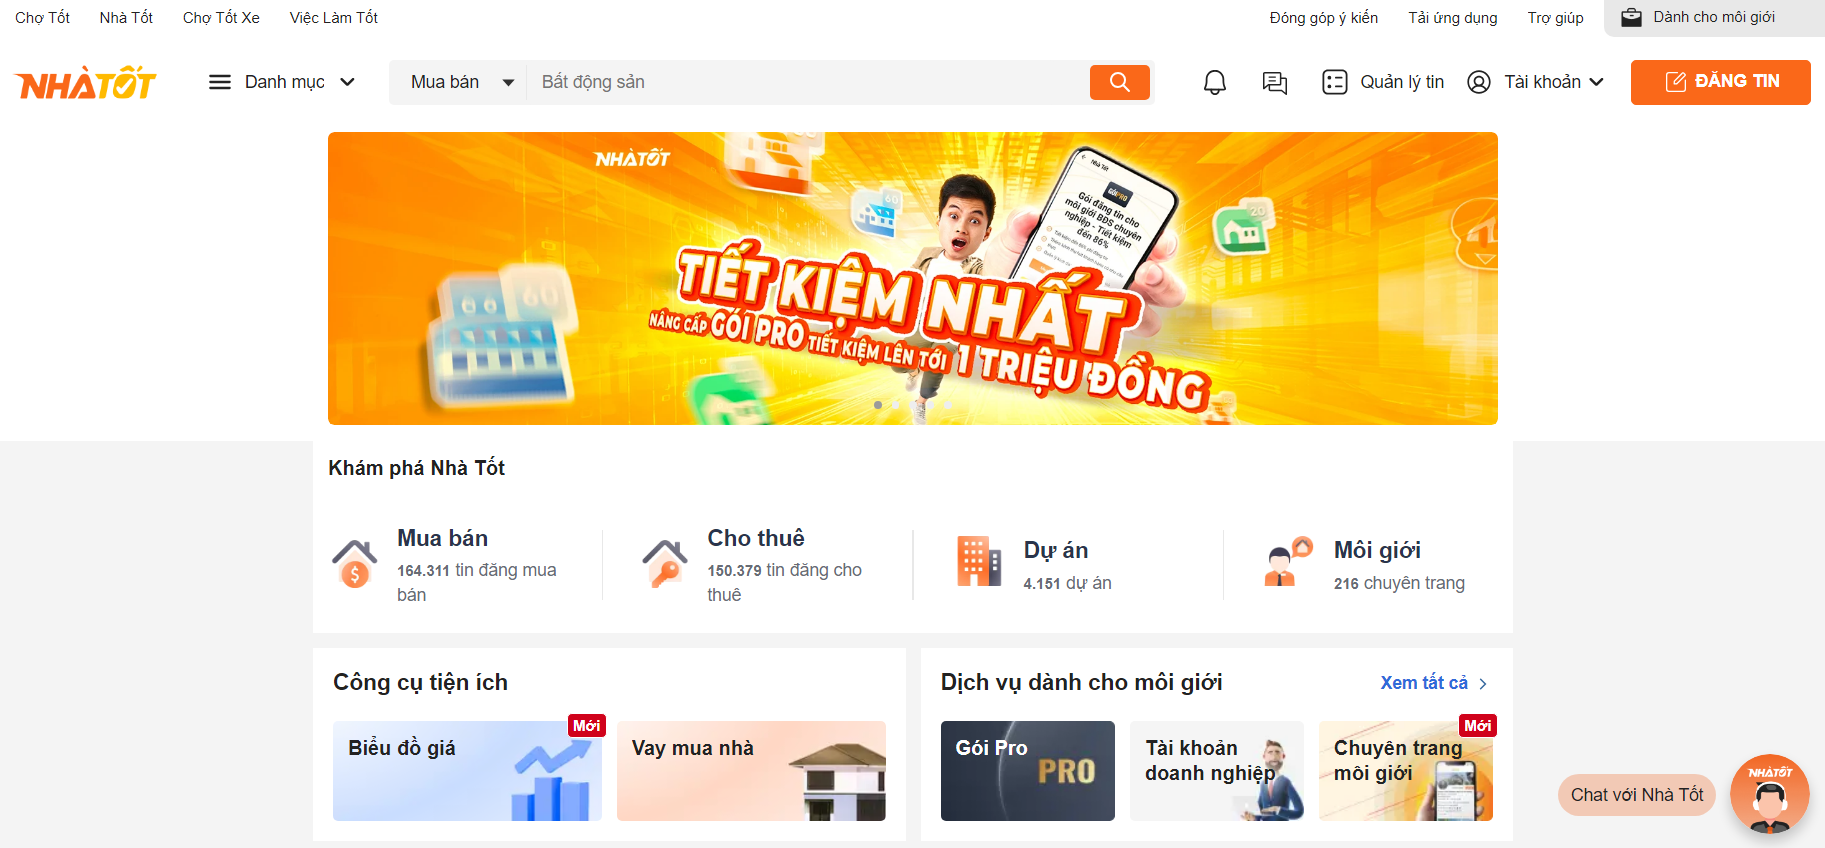
\includegraphics[width=1\textwidth]{Images/RelatedSystems/NhatotDesktop.png}
    \caption{Giao diện Nhà Tốt trên website}
\end{figure}
\begin{figure}[H]
    \centering
    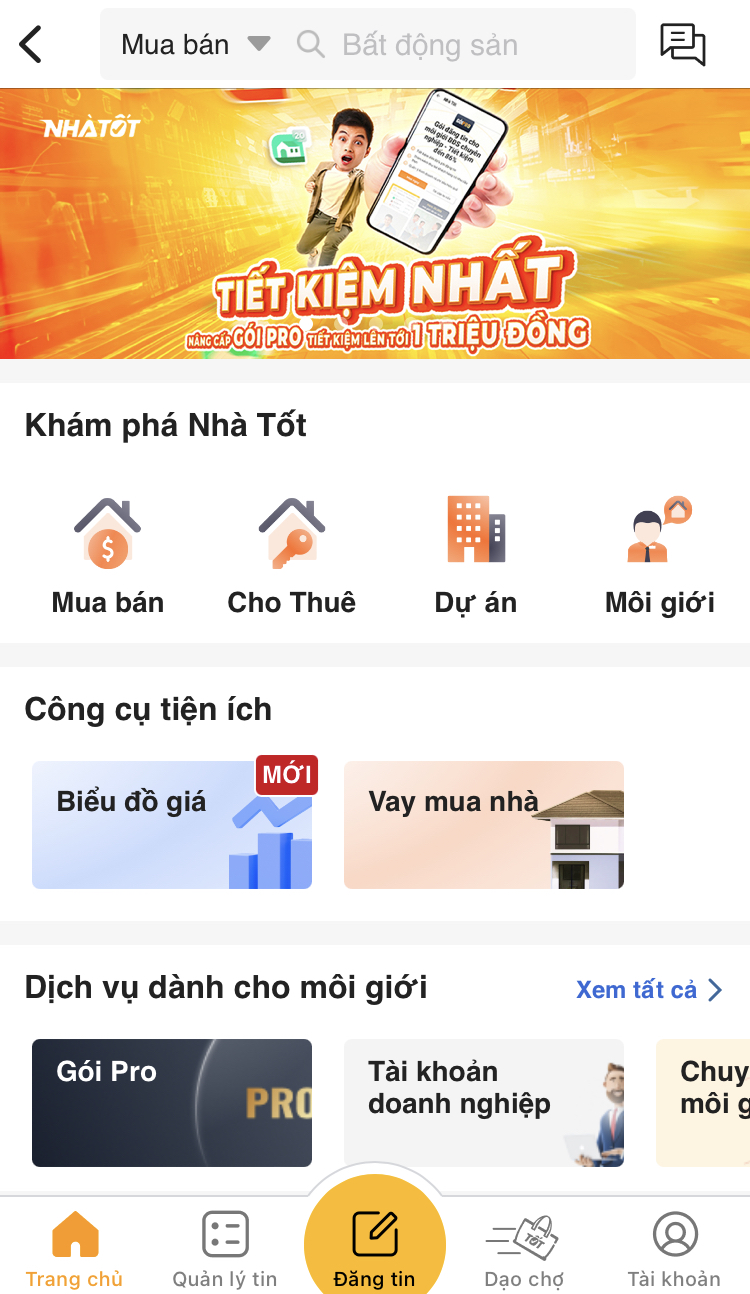
\includegraphics[width=0.5\textwidth]{Images/RelatedSystems/NhatotMobile.PNG}
    \caption{Giao diện Nhà Tốt trên thiết bị di động}
\end{figure}
\subsection{Các tính năng chính}
Nhà Tốt là một nền tảng trực tuyến kết nối người mua, người bán, và những người quan tâm đến thị trường bất động sản. Dưới đây là một số tính năng chính của Nhà Tốt:
\begin{itemize}
    \item \textbf{Tìm kiếm bất động sản}
    \begin{itemize}
        \item \textit{Tìm kiếm theo vị trí:} Người sử dụng có thể tìm kiếm bất động sản theo vị trí cụ thể, chẳng hạn như thành phố, quận, phường
        \item \textit{Phân loại theo danh mục:} Phân loại bất động sản mua bán, cho thuê, tìm kiếm các dự án đang được phát triển
        \item \textit{Bộ lọc nâng cao}: Lọc các kết quả bất động sản tìm được dựa trên khoảng giá, diện tích, số phòng.
    \end{itemize}
    \item \textbf{Đăng tải bất động sản}
    \begin{itemize}
        \item \textit{Đăng tin bất động sản:} Người dùng có thể đăng tải bài đăng về cho thuê hoặc mua bán bất động sản, có thể cung cấp các hình ảnh trực quan về bất động sản và các thông tin chi tiết khác để người dùng dễ tiếp cận
        \item \textit{Quản lý tin đăng:} Người dùng quản lý tin đăng thông qua việc chỉnh sửa bài đăng hoặc có thể gỡ bỏ bài đăng bất động sản.
    \end{itemize}
    \item \textbf{Tương tác giữa người mua và người bán:}
    \begin{itemize}
        \item \textit{Số điện thoại liên hệ:} Người đăng sẽ để lại số điện thoại liên hệ trên bài đăng và khi có nhu cầu, người mua hoặc thuê sẽ gọi đến người đăng thông qua số điện thoại đó.
        \item \textit{Trò chuyện trực tiếp:} Người đăng và người mua hoặc thuê có thể nhắn tin trực tiếp với nhau thông qua ứng dụng.
        \item \textit{Gửi câu hỏi:} Người mua hoặc thuê cũng có thể để lại câu hỏi và đợi người đăng phản hồi lại trong một khoảng thời gian.
    \end{itemize}
    \item \textbf{Trung tâm trợ giúp}:
    \begin{itemize}
        \item \textit{Hướng dẫn:} Nhà Tốt cung cấp các hướng dẫn chi tiết dành cho người mua và người bán trên ứng dụng, họ có thể tiếp cận những hướng dẫn để giúp cho việc trải nghiệm trên ứng dụng được hiệu quả hơn
        \item \textit{Các câu hỏi phổ biến:} Người dùng có thể tìm kiếm nhanh chóng những vấn đề phổ biến thường gặp khi trải nghiệm ứng dụng và giải đáp cho những vấn đề đó.
        \item \textit{Trò chuyện trực tiếp:} Bất cứ lúc nào, người dùng có thể liên lạc trực tiếp với trợ lý ảo của chợ tốt để giải đáp cụ thể những thắc mắc hay những vấn đề có thể gặp phải
    \end{itemize}
\end{itemize}
\subsection{Phân Tích SWOT}
\begin{tcbraster}[raster columns=2, boxrule=0mm, arc=0mm]
\begin{tcolorbox}[equal height group=A, size=fbox, colback=swotS!60, colframe=swotS!80!black, title=\textsc{strengths}]
\begin{itemize}
\item Nhà Tốt là một thương hiệu bất động sản uy tín, được nhiều người biết đến. Thương hiệu này đã được xây dựng trong nhiều năm qua, thông qua các hoạt động quảng bá tích cực, cũng như chất lượng dịch vụ tốt.
\item Nhà Tốt có lượng người truy cập lớn, đa dạng, bao gồm cả người mua, người bán và các nhà đầu tư bất động sản. Điều này cho thấy website của Nhà Tốt đã thu hút được sự quan tâm của nhiều đối tượng khách hàng.
\end{itemize}
\end{tcolorbox}
\begin{tcolorbox}[equal height group=A, size=fbox, colback=swotW!60, colframe=swotW!80!black, title=\textsc{weaknesses}]
\begin{itemize}
\item Nội dung website của Nhà Tốt chưa được cập nhật thường xuyên, khiến cho website trở nên thiếu cập nhật, thiếu hấp dẫn.
\item Trải nghiệm người dùng trên website của Nhà Tốt chưa được tối ưu, khiến cho người dùng gặp khó khăn trong việc tìm kiếm thông tin, sử dụng các tính năng trên website.
\item Nhà Tốt chưa có nhiều tính năng mới, hấp dẫn, đáp ứng nhu cầu của người dùng.
\item Nhà Tốt chưa tận dụng được sức mạnh của các kênh truyền thông xã hội để tiếp cận với nhiều khách hàng hơn.
\end{itemize}
\end{tcolorbox}
\begin{tcolorbox}[equal height group=B, size=fbox, colback=swotO!60, colframe=swotO!80!black, title=\textsc{opportunities}]
\begin{itemize}
\item Thị trường bất động sản Việt Nam đang phát triển mạnh mẽ, tạo ra nhiều cơ hội cho các trang web bất động sản. Nhu cầu tìm kiếm nhà đất của người dân ngày càng tăng, tạo ra nhiều tiềm năng cho các trang web bất động sản.
\item Công nghệ đang phát triển, tạo ra nhiều cơ hội mới cho các trang web bất động sản, như: phát triển các tính năng mới, hấp dẫn, tối ưu trải nghiệm người dùng,...
\item Tăng trưởng của các kênh thương mại điện tử tạo ra cơ hội cho các trang web bất động sản mở rộng hoạt động kinh doanh của mình sang các lĩnh vực khác như: môi giới, tư vấn bất động sản,...
\end{itemize}
\end{tcolorbox}
\begin{tcolorbox}[equal height group=B, size=fbox, colback=swotT!60, colframe=swotT!80!black, title=\textsc{threats}]
\begin{itemize}
\item Sự cạnh tranh ngày càng gay gắt từ các trang web bất động sản khác, khiến cho Nhà Tốt cần phải nỗ lực hơn nữa để giữ vững vị thế của mình.
\item Thị trường bất động sản thay đổi nhanh chóng, khiến cho Nhà Tốt cần phải cập nhật thông tin thường xuyên, để cung cấp cho khách hàng những thông tin chính xác, kịp thời.
\item Luật pháp, quy định liên quan đến bất động sản có thể thay đổi, khiến cho Nhà Tốt cần phải cập nhật những thay đổi này, để đảm bảo tuân thủ đúng quy định.
\end{itemize}
\end{tcolorbox}
\captionof{table}{Phân tích SWOT cho Nhà Tốt}
\end{tcbraster}
\subsection{Nhận xét}
\hspace*{1cm}Nhà Tốt không chỉ là một ứng dụng tìm kiếm bất động sản thông thường, mà còn là nơi kết nối cộng đồng bất động sản, tạo ra một môi trường tương tác động và tích cực. Giao diện trực quan và tiện ích đa dạng của ứng dụng tạo ra một trải nghiệm người dùng linh hoạt và thú vị, đồng thời tạo ra một giải pháp tiện lợi nhanh chóng trong việc giao dịch bất động sản.\\
\hspace*{1cm}Một điểm mạnh lớn của Nhà Tốt là khả năng kết nối người mua và người bán một cách nhanh chóng và thuận lợi. Hệ thống thông tin đầy đủ và chính xác giúp người mua hiểu rõ hơn về các bất động sản, từ đó đưa ra quyết định mua bán chính xác và linh hoạt. Hơn nữa, việc tận dụng công nghệ để cung cấp thông tin thị trường và xu hướng giúp người dùng nắm bắt tốt hơn về cơ hội đầu tư và phát triển. Sự đổi mới không chỉ là về trải nghiệm người dùng mà còn về mô hình kinh doanh. Nhà Tốt có thể tận dụng mạng lưới xã hội để xây dựng uy tín và đánh giá cộng đồng, tạo ra sự minh bạch và tin cậy trong quá trình giao dịch bất động sản.\\
\hspace*{1cm}Tuy nhiên, Nhà Tốt cũng phải đối mặt với những thách thức, như cạnh tranh khốc liệt từ các đối thủ cũng như việc quản lý vấn đề pháp lý và thuế. Điều này đòi hỏi sự tập trung và linh hoạt từ đội ngũ quản lý để đảm bảo bền vững trong hoạt động kinh doanh.Tóm lại, sự xuất hiện của Nhà Tốt không chỉ là một thách thức mà còn là cơ hội để nâng cao chất lượng dịch vụ và đáp ứng nhu cầu đa dạng của thị trường bất động sản ngày càng phát triển tại Việt Nam.